%% witnessfinding.tex - Lower bounds for witness-finding algorithms
%%
%% Copyright 2014 Jeffrey Finkelstein.
%%
%% This LaTeX markup document is made available under the terms of the Creative
%% Commons Attribution-ShareAlike 4.0 International License,
%% https://creativecommons.org/licenses/by-sa/4.0/.
\documentclass{article}

\usepackage{amsmath}
\usepackage{amssymb}
%% This must come before hyperref.
\usepackage{amsthm}
%% This is strongly recommended by biblatex.
\usepackage[english]{babel}
\usepackage[backend=biber]{biblatex}
\usepackage[T1]{fontenc}
%% This must come before csquotes.
\usepackage[utf8]{inputenc}
\usepackage{lmodern}
%% This is strongly recommended by biblatex.
\usepackage{csquotes}
%% This must come before hyperref.
\usepackage{thmtools}
%% This must come before complexity.
\usepackage{hyperref}
\usepackage{complexity}
\usepackage[firstpage]{draftwatermark}
\usepackage{microtype}
\usepackage{textcomp}
\usepackage{tikz}

\LoadMicrotypeFile{cmr}
\SetProtrusion
    [load=lmr-T1]
    {encoding=T1, family=lmr}
    {
      \textquotedblright = {,1000},
      \textquotedblleft = {1000,},
      {'} = {,1000},
      {[} = {1000,},
      {]} = {,1000},
      {,} = {,1000},
      {:} = {,1000},
      {;} = {,1000},
      {.} = {,1000}
    }

%% Set the ``work-in-progress'' watermark for the first page.
\SetWatermarkLightness{0.9}
\SetWatermarkText{Work-in-progress}
\SetWatermarkFontSize{3.5cm}

\hypersetup{pdftitle={Lower bounds for witness-finding algorithms}, pdfauthor={Jeffrey Finkelstein}}

\addbibresource{witnessfinding.bib}

\declaretheorem[numberwithin=section]{theorem}
\declaretheorem[numberlike=theorem]{lemma}
\declaretheorem[numberlike=theorem]{proposition}
\declaretheorem[numberlike=theorem]{corollary}
\declaretheorem[numberlike=theorem]{conjecture}
\declaretheorem[numberlike=theorem, style=definition]{definition}

%% Custom commands are declared here.
\newcommand{\email}[1]{\textlangle\href{mailto:#1}{\nolinkurl{#1}}\textrangle}
\newcommand{\todo}[1]{\textbf{TODO #1}}
\newcommand{\mc}{\mathcal}
\newcommand{\floor}[1]{\left\lfloor{#1}\right\rfloor}
\newcommand{\ceil}[1]{\left\lceil{#1}\right\rceil}
\DeclareMathOperator{\pow}{pow}
\newcommand{\mono}{\mathsf{mono}}
\newcommand{\direct}{\mathsf{direct}}
\newcommand{\all}{\mathsf{all}}

%% Redefine the footnote environment so it has no reference and no number.
\long\def\symbolfootnote#1{\begingroup%
\def\thefootnote{\fnsymbol{footnote}}\footnotetext{#1}\endgroup}

\title{Lower bounds for witness-finding algorithms}
\author{Jeffrey Finkelstein}

\begin{document}

\maketitle

\symbolfootnote{%
  Copyright 2014 Jeffrey~Finkelstein \email{jeffreyf@bu.edu}.

  This document is licensed under the Creative Commons Attribution-ShareAlike 4.0 International License, which is available at \mbox{\url{https://creativecommons.org/licenses/by-sa/4.0/}}.
  The \LaTeX{} markup that generated this document can be downloaded from its website at \mbox{\url{https://github.com/jfinkels/witnessfinding}}.
  The markup is distributed under the same license.
}

\section{Introduction}
%%
%% context
Can a procedure that decides whether a Boolean formula has a satisfying assignment help to find such an assignment?
The naïve adaptive ``search-to-decision'' reduction uses a linear number of (quite weak) queries.
%% need
Is there a lower bound on the number of queries required for a nonadaptive search-to-decision reduction?
%% task
We report on lower bounds for various classes of queries.
%% object

%% findings
Most interesting types of queries require at least $\Omega(n^2)$ queries to find a witness.
%% conclusion
We were hoping to use lower bounds on these types of witness-finding algorithms to show that randomized reductions to $\CeP$ are less powerful than randomized reductions to $\PP$, but we were unable to do so.
%% perspectives

\autoref{fig:queries} contains a summary of the upper and lower bounds for nonadaptive witness-finding algorithms.
In addition, adaptive $\mc{Q}_0$ algorithms use $\Theta(n)$ queries, and adaptive $\mc{Q}_1$ witness-finding algorithms with high success probability use $\Theta(n^2)$ queries.
\todo{Currently the lower bound for the query complexity of adaptive $\mc{Q}_1$ witness-finding algorithms with success probability $\frac{1}{2}$ is $\Omega(n)$.
  Can we either improve this to $\Omega(n^2)$ or provide a $O(n)$ upper bound?
}

\todo{Compare these randomized witness-finding algorithms with ``bounded query hierarchy'' algorithms, in which the query generator and the witness generator are not randomized (but possibly nondeterministic), and the goal is to decide a language, not necessarily output a witness.}

\begin{figure}
  \caption{\label{fig:queries}%
    When considering nonadaptive witness-finding algorithms, $\mc{Q}_{\direct}$ algorithms require $\Omega(2^n)$ queries, $\mc{Q}_{\mono}$, $\mc{Q}_{\NP}$, and $\mc{Q}_k$ algorithms require $\Omega(n^2)$ queries, and $\mc{Q}_{\all}$ algorithms require $\Omega(n)$ queries.
    In this diagram, lower bounds propagate downward and upper bounds propagate upward.%
  }
  \begin{center}
    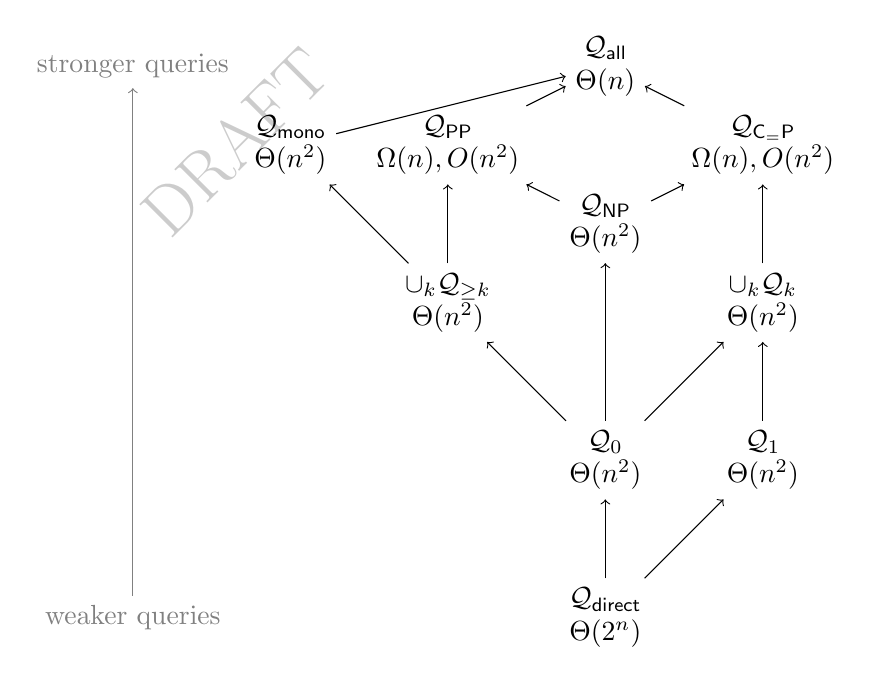
\begin{tikzpicture}[->, every node/.style={align=center}]
      \node at (0, 0) (direct) {$\mc{Q}_{\direct}$ \\ $\Theta(2^n)$};
      \node at (0, 2) (equal0) {$\mc{Q}_0$ \\ $\Theta(n^2)$};
      \node at (2, 2) (equal1) {$\mc{Q}_1$ \\ $\Theta(n^2)$};
      \node at (0, 5) (NP) {$\mc{Q}_{\NP}$ \\ $\Theta(n^2)$};
      \node at (-2, 4) (geqk) {$\cup_k \mc{Q}_{\geq k}$ \\ $\Theta(n^2)$};
      \node at (2, 4) (eqk) {$\cup_k \mc{Q}_k$ \\ $\Theta(n^2)$};
      \node at (-2, 6) (PP) {$\mc{Q}_{\PP}$ \\ $\Omega(n), O(n^2)$};
      \node at (2, 6) (CeP) {$\mc{Q}_{\CeP}$ \\ $\Omega(n), O(n^2)$};
      \node at (-4, 6) (mono) {$\mc{Q}_{\mono}$ \\ $\Theta(n^2)$};
      \node at (0, 7) (all) {$\mc{Q}_{\all}$ \\ $\Theta(n)$};
      \draw (direct) to (equal0);
      \draw (direct) to (equal1);
      \draw (equal0) to (NP);
      \draw (equal0) to (geqk);
      \draw (equal0) to (eqk);
      \draw (equal1) to (eqk);
      \draw (eqk) to (CeP);
      \draw (geqk) to (PP);
      \draw (geqk) to (mono);
      \draw (NP) to (CeP);
      \draw (NP) to (PP);
      \draw (PP) to (all);
      \draw (mono) to (all);
      \draw (CeP) to (all);

      \node[color=gray] at (-6, 0) (weak) {weaker queries};
      \node[color=gray] at (-6, 7) (strong) {stronger queries};
      \draw[color=gray] (weak) to (strong);
    \end{tikzpicture}
  \end{center}
\end{figure}

\section{Definitions}

Let $\Sigma = \{0, 1\}$.
For any natural number $n$, the set $\Sigma^n$ denotes the set of binary strings of length $n$.
For each $b \in \{0, 1\}$, let $\bar{b} = 1 - b$.
Let $[n] = \{1, \dotsc, n\}$.
Denote by $\log n$ the base-$2$ logarithm.

A language $L \subseteq \Sigma^*$ is a \emph{witnessed language} if there exists a language $L' \subseteq \Sigma^* \times \Sigma^*$, called the \emph{witness relation}, such that for each $x$ of length $n$, we have $x \in L$ if and only if there is a $w \in \Sigma^n$ such that $(x, w) \in L'$.
(We don't consider strings $w$ of length polynomial in $n$ because a language in any ``well-behaved'' complexity class can be converted to an equivalent language in which all witnesses have length exactly $n$ by padding the string $x$ by an appropriate amount.)

Suppose $n$ is a positive integer.
A \emph{witness set} is a nonempty subset of $\Sigma^n$ denoted by $W$, and each element of $W$ is a \emph{witness}.
A \emph{query} is a Boolean predicate $Q \colon \pow(\Sigma^n) \to \{0, 1\}$.

\begin{definition}[{\autocite{krw14}}]
  Let $\mc{W}$ be a collection of witness sets and $\mc{Q}$ a collection of queries.
  A \emph{(nonadaptive) $\mc{Q}$-query witness-finding algorithm} is a joint distribution $(Q_1, \dotsc, Q_m)$ on $\mc{Q}^m$, for some natural number $m$, and a function $f \colon \{0, 1\}^m \to \Sigma^n$ such that $\Pr[f(Q_1(W), \dotsc, Q_m(W)) \in W] > \frac{1}{2}$ for each $W \in \mc{W}$.
  The number $m$ is the \emph{query complexity} of the algorithm.
\end{definition}

This definition can be generalized to allow for success probabilities other than $\frac{1}{2}$, and to allow for adaptive queries.
Unless otherwise specified, the success probability is assumed to be $\frac{1}{2}$ and the queries are assumed to be nonadaptive.

\todo{Define an ``adaptive distribution sequence'' (which means that $Q_{i + 1}(W)$ is actually $Q_{i + 1}(W, Q_1(W), \dotsc, Q_{i - 1}(W))$).}

\begin{itemize}
\item
  An \emph{$(= k)$ query} is a query $Q_S$ of the form $Q_{S}(W) = 1$ if and only $|S \cap W| = k$, for any $S \subseteq \Sigma^n$ and any $W \in \pow(\Sigma^n)$.
  The collection of all $(= k)$ queries is denoted $\mc{Q}_k$.
\item
  A \emph{$(\geq k)$ query} is a query $Q_S$ of the form $Q_{S}(W) = 1$ if and only $|S \cap W| \geq k$, for any $S \subseteq \Sigma^n$ and any $W \in \pow(\Sigma^n)$.
  The collection of all $(\geq k)$ queries is denoted $\mc{Q}_{\geq k}$.
\item
  An element of $\mc{Q}_1$ is called an \emph{isolation query}.
\item
  An element of $\mc{Q}_0$ is called an \emph{emptiness query}.
\end{itemize}

\begin{definition}
  Let $\mc{W}$ be a collection of witness sets.
  A \emph{hitting algorithm} is an adaptive sequence of distributions $(Q_1, \dotsc, Q_m)$ on $\mc{Q}^m_1$, for some natural number $m$, such that $\Pr[Q_m(W) = 1] > \frac{1}{2}$.
  The number $m$ is the \emph{query complexity} of the algorithm.
\end{definition}

This definition is a complexity theoretic restatement of the combinatorial ``hitting game'', as described in \autocite[Section~3]{newport14} (the original definition seems to be from \autocite[Definition~5]{bgi92}).

A hitting algorithm is always an adaptive algorithm; a nonadaptive hitting algorithm makes little sense here because it would be essentially the same as simply guessing an element of the witness set at random.

A witness-finding algorithm must output an element of $W$, whereas a hitting algorithm need not.

\todo{define polynomial-time algorithms (provide polysize circuits that encode the query sets)}

\section{Relationship among algorithms}

\begin{proposition}\label{prop:flip}
  Let $k$ be a positive integer.
  \begin{itemize}
  \item There is a $\mc{Q}_{\geq k}$ witness-finding algorithm if and only if there is a $\mc{Q}_{< k}$ witness-finding algorithm.
  \item There is a $\mc{Q}_k$ witness-finding algorithm if and only if there is a $\mc{Q}_{\neq k}$ witness-finding algorithm.
  \end{itemize}
  Furthermore, in both cases, the query complexity of the algorithms is exactly the same.
\end{proposition}
\begin{proof}
  We prove the first equivalence; the second is similar.
  For each $Q_S$ in $\mc{Q}_{\geq k}$ there is a corresponding $\overline{Q_S}$ in $\mc{Q}_{< k}$ such that $\overline{Q_S(W)} = \overline{Q_S}(W)$ for each witness set $W$, and furthermore, this correspondence is a bijection.
  Therefore if we define the function $\bar{f}$ by
  \begin{equation*}
    \bar{f}(A_1, \dotsc, A_m) = f(\overline{A_1}, \dotsc, \overline{A_m}),
  \end{equation*}
  for all possible bits $A_1, \dotsc, A_m$, we get the desired equivalence: $((Q_1, \dotsc, Q_m), f)$ is equivalent to $((Q_1, \dotsc, Q_m), \bar{f})$.
\end{proof}

\begin{corollary}\label{cor:flip}
  There is a $\mc{Q}_0$ witness-finding algorithm if and only if there is a $\mc{Q}_{\neq 0}$ witness-finding algorithm.
\end{corollary}

\begin{proposition}\label{prop:leqgeq}
  Let $k$ and $m$ be natural numbers.
  If there is a $\mc{Q}_k$ witness-finding algorithm with query complexity $m$, then there is a $\mc{Q}_{\geq k} \cup \mc{Q}_{\geq k + 1}$ witness-finding algorithm with query complexity $2 m$.
\end{proposition}
\begin{proof}
  Suppose $((Q_{S_1}, \dotsc, Q_{S_m}), f)$ is the $\mc{Q}_k$ witness-finding algorithm.
  By \autoref{prop:flip}, it suffices to show a $\mc{Q}_{\geq k} \cup \mc{Q}_{\leq k}$ witness-finding algorithm.
  For each $Q_{S_i}$, construct two queries $Q^\geq_{S_i}$ and $Q^\leq_{S_i}$ defined as $Q^\geq_{S_i}(W) = 1$ if and only $|S_i \cap W| \geq k$ and $Q^\leq_{S_i}(W) = 1$ if and only if $|S_i \cap W| \leq k$.
  Define $f'$ by
  \begin{equation*}
    f'(A_1, \dotsc, A_m, B_1, \dotsc, B_m) = f(A_1 \land B_1, \dotsc, A_m \land B_m),
  \end{equation*}
  for all bits $A_1, \dotsc, A_m$ and all bits $B_1, \dotsc, B_m$.
  Since $Q^\geq_{S_i}(W) \land Q^\leq_{S_i}(W) = Q_{S_i}(W)$, the correctness of $((Q^\geq_{S_1}, \dotsc Q^\geq_{S_m}, Q^\leq_{S_1}, \dotsc, Q^\leq_{S_m}), f')$ follows from the correctness of $((Q_1, \dotsc, Q_m), f)$.
\end{proof}

The problem of finding a hitting algorithm reduces to the problem of finding a $\mc{Q}_1$ witness-finding algorithm.

\begin{lemma}\label{lem:reduction}
  Let $m$ be a natural number.
  If there is a $\mc{Q}_1$ witness-finding algorithm with query complexity $m$, then there is a hitting algorithm with query complexity $m + 1$.
\end{lemma}
\begin{proof}
  Suppose $((Q_{S_1}, \dotsc, Q_{S_m}), f)$ is the $\mc{Q}_1$ witness-finding algorithm.
  For any witness set $W$, let $S_{m + 1}$ be the singleton set containing the element $f(Q_{S_1}, \dotsc, Q_{S_m})$.
  Then $(Q_{S_1}, \dotsc, Q_{S_{m + 1}})$ is a hitting algorithm, since the probability that $f(Q_{S_1}(W), \dotsc, Q_{S_m}(W)) \in W$ is exactly the probability that $Q_{S_{m + 1}}(W) = 1$.
\end{proof}

On the other hand, there does not seem to be a general reduction from a $\mc{Q}_1$ witness-finding algorithm to a hitting algorithm.
In order to output a single witness knowing only that a witness is contained in a particular query set doesn't help, unless the query set is small; there is no such guarantee on the size of that set.

\begin{conjecture}\label{conj:hitting}
  Under an appropriate setting of parameters, if the existence of a hitting algorithm implies the existence of an isolation query algorithm, then $\RP = \NP$.
  \todo{But both types of algorithms exist with the same parameters, as shown in the next section.}
\end{conjecture}

Now, consider the possibility that a $\mc{Q}_k$ witness-finding algorithm implies a $\mc{Q}_{k - 1}$ witness-finding algorithm.
Intuitively, in order for this to work, the latter algorithm would have to simulate the queries $Q_i$ from the former algorithm with some sort of collection of queries of the form $Q_i \setminus \{q_{i, j}\}$, where $q_{i, j}$ is the $j$th member of $Q_i$.
However, the oracle answers would be inconsistent, because we don't know beforehand whether $q_{i, j}$ is in the witness set or not (causing a discrepancy between the answers of the two oracles).
A similar problem arises when attempting the converse simulation: the simulated queries would be something of the form $Q_i \cup \{v_j\}$, where $v_j$ is the $j$th element of $\Sigma^n \setminus Q_i$, thus there would be a discrepancy between the answers of the two oracles.
We therefore conjecture that there is evidence that such a simulation is unlikely.

\begin{conjecture}\label{conj:ktokplus1}
  For each $k \in \left[2^n\right]$, if the existence of a $\mc{Q}_k$ witness-finding algorithm implies the existence of a $\mc{Q}_{k + 1}$ witness-finding algorithm, then $\RP = \NP$.
  \todo{But both such algorithms exist unconditionally, as shown in the next section.}
\end{conjecture}

\section{Upper bounds}

\begin{theorem}\label{thm:naive}
  There is a polynomial time adaptive $\mc{Q}_0$ witness-finding algorithm with success probability $1$ and query complexity $O(n)$.
\end{theorem}
\begin{proof}[Proof idea]
  By \autoref{cor:flip}, it suffices to show a $\mc{Q}_{\neq 0}$ witness-finding algorithm.
  This the well-known bit-by-bit $\P^\NP$ computable function for computing a witness for a given string.

  For each $i \in [n]$ and each $b \in \{0, 1\}$, define the query $S_{i, b}$ inductively (or in other words, adaptively) as follows.
  If $i = 1$, then $S_{i, b} = \{ b v \, | \, v \in {\{0, 1\}}^{n - 1}\}$.
  For each subsequent pair of queries, let $u = b_1 \dotsb b_{i - 1}$, where $b_j$ is a bit that caused the oracle to answer ``yes'' on query $S_{j, b_j}$ for each $j \in [i - 1]$, and let $S_{i, b} = \{ u b v \, | \, v \in {\{0, 1\}}^{n - i}\}$.
  Finally, given the responses to $S_{n, 0}$ and $S_{n, 1}$, which are singleton sets, the algorithm simply outputs the sole element of the query set that caused the oracle to answer ``yes''.

  The total number of queries is $2n$, which is in $O(n)$.
\end{proof}

This upper bound means that any class of queries containing $\mc{Q}_0$ as a subset also satisfies this very strong upper bound.

\begin{theorem}[{\autocite[Theorem~1.4]{krw14} (citing \autocite{bcgl92})}]\label{thm:vv}
  There is a polynomial time $\mc{Q}_0$ witness-finding algorithm with query complexity $O(n^2)$.
\end{theorem}
\begin{proof}[Proof idea]
  By \autoref{cor:flip}, it suffices to show a $\mc{Q}_{\neq 0}$ witness-finding algorithm.
  This algorithm uses the Valiant--Vazirani Isolation Lemma in each query to guess each bit of a possible witness (in parallel).

  First, consider a simpler set of queries.
  Let $s$ be a string in $\Sigma^r$.
  For each $i \in [n]$ and each $b \in \Sigma$, let $S_{i, b} = \{ w \, | \, w \in C_s \land w_i = b\}$, where $C$ is the isolating set from the Valiant--Vazirani Isolation Lemma (for example, the set of all strings whose image is zero under a pairwise independent hash function).
  The Valiant--Vazirani Isolation Lemma proves that this algorithm has success probability $\Omega(\frac{1}{n})$ and query complexity $O(n)$.
  In order to get success probability $\Omega(1)$, we create $O(n)$ collections of $O(n)$ queries, with an independent set $C_{s_k}$ for each collection.
  Now our queries are $S_{k, i, b} = \{ w \, | \, w \in C_{s_k} \land w_i = b\}$, for each $k \in \left[O(n)\right]$, each $i$, and each $b$.
\end{proof}

In \autocite{krw12}, the authors call the above theorem the ``truth-table reduction'' analog of the ``many-one reduction'' result of \autocite[Theorem~4.2]{dkvmw13}.
However, this is not strictly precise, since the former involves $\mc{Q}_0$ queries, whereas the latter involves $\mc{Q}_1$ queries.
Fortunately, the proof uses the Valiant--Vazirani Isolation Lemma (that is, the sets $C_{s_k}$), so the probability that $|S \cap W| \neq 0$ equals the probability that $|S \cap W| = 1$.
(On the other hand, there is no other known relationship between $\mc{Q}_0$ witness-finding algorithms and $\mc{Q}_1$ witness-finding algorithms, other than the fact that $\mc{Q}_0 \cup \mc{Q}_1 \subseteq \cup_{k \in \mathbb{N}} \mc{Q}_k$.)

\begin{corollary}\label{cor:q1upper}
  There is a polynomial time $\mc{Q}_1$ witness-finding algorithm with query complexity $O(n^2)$.
\end{corollary}

\todo{Double check this logic.}

\begin{corollary}
  There is a polynomial time hitting algorithm with query complexity $O(n^2)$.
\end{corollary}
\begin{proof}
  Combine the previous corollary with \autoref{lem:reduction}.
\end{proof}

\section{Lower bounds}

A query $Q$ is a \emph{monotone query} if for all $W$ and $W'$, subsets of $\Sigma^n$, if $W \subseteq W'$, then $Q(W) = 1$ implies $Q(W') = 1$.
The collection of all monotone queries is denoted $\mc{Q}_{\mono}$.

\begin{theorem}[{\autocite[Theorem~1.3]{krw14}}]\label{thm:monotonelower}
  Each $\mc{Q}_{\mono}$ witness-finding algorithm has query complexity $\Omega(n^2)$.
\end{theorem}

The proof of this theorem relies on the existence of a distribution on witness sets that places all witnesses far apart, so it is hard to guess both the number and location of the witnesses.
This distribution comes from \autocite[Theorem~4.2]{dkvmw13}.

An infinite sequence of queries $(Q^1, Q^2, \dotsc)$ is an \emph{$\NP$ query} if there is a nondeterministic oracle Turing machine $M$ such that for each $n$, we have $Q^n(W) = 1$ if and only if $M^W(1^n)$ accepts (where $Q^n$ denotes a query on witness sets of strings of size $n$).
The collection of all $\NP$ queries is denoted $\mc{Q}_{\NP}$.

\begin{theorem}[{\autocite[Theorem~1.6]{krw14}}]\label{thm:nplower}
  Each $\mc{Q}_{\NP}$ witness-finding algorithm has query complexity $\Omega(n^2)$.
\end{theorem}

\begin{corollary}[{\autocite[Theorem~2]{krw12}}]\label{cor:q0lower}
  Each $\mc{Q}_0$ witness-finding algorithm has query complexity $\Omega(n^2)$.
\end{corollary}
\begin{proof}
  This is a special case of both \autoref{thm:monotonelower} and \autoref{thm:nplower}.
\end{proof}

The next corollary is a generalization of \autocite[Remark~2]{krw12}.

\begin{corollary}\label{cor:geqk}
  Suppose $k \in \left[2^n\right]$.
  Each $\mc{Q}_{\geq k}$ witness-finding algorithm has query complexity $\Omega(n^2)$.
\end{corollary}
\begin{proof}
  This is a special case of \autoref{thm:monotonelower}.
\end{proof}

\begin{corollary}\label{cor:equalsk}
  Suppose $k \in \left[2^n\right]$.
  Each $\mc{Q}_k$ witness-finding algorithm has query complexity $\Omega(n^2)$.
\end{corollary}
\begin{proof}
  This is a proof by contradiction.
  Assume there is a $\mc{Q}_k$ witness-finding algorithm with query complexity $o(n^2)$.
  By \autoref{prop:leqgeq}, there is a $\mc{Q}_{\geq k} \cup \mc{Q}_{\geq k + 1}$ witness-finding algorithm with query complexity $o(n^2)$.
  Since $\mc{Q}_{\geq k}$ and $\mc{Q}_{\geq k + 1}$ are both subsets of the collection of all monotone queries, each $\mc{Q}_{\geq k} \cup \mc{Q}_{\geq k + 1}$ witness-finding algorithm has query complexity $\Omega(n^2)$, by \autoref{thm:monotonelower}.
  This is a contradiction.
\end{proof}

\begin{corollary}\label{cor:q1lower}
  Each $\mc{Q}_1$ witness-finding algorithm has query complexity $\Omega(n^2)$.
\end{corollary}
\begin{proof}
  This is a special case of the previous corollary.
\end{proof}

\begin{theorem}[{\autocite[Theorems~3.3 and 3.4]{newport14}}]
  Each hitting algorithm with success probability $\Omega(1 - 2^{-n})$ has query complexity $\Omega(n^2)$.
  Furthermore, this is true even when restricted to witness sets of cardinality two.
\end{theorem}

The proof of this theorem relies on the probabilistic method to show the existence of a witness set that is hard to ``hit'', found in \autocite{ablp91}.

\begin{corollary}\label{cor:isolationalg}
  Each adaptive $\mc{Q}_1$ isolation query algorithm with success probability $\Omega(1 - 2^{-n})$ has query complexity $\Omega(n^2)$.
  Furthermore, this is true even when restricted to witness sets of cardinality two.
\end{corollary}
\begin{proof}
  This is a proof by contradiction.
  Assume there is an adaptive $\mc{Q}_1$ witness-finding algorithm with success probability $\Omega(1 - 2^{-n})$ and query complexity $o(n^2)$.
  By \autoref{lem:reduction}, there is a hitting algorithm with the same success probability and query complexity (up to constant factors).
  This would contradict the previous theorem, hence no such algorithm exists.
\end{proof}

%% We know that for adaptive $\mc{Q}_0$ witness-finding algorithms, there is a query complexity upper bound of $O(n)$ (see \autoref{thm:naive}), matching the lower bound of $\Omega(n)$.
%% Since we don't know whether $\mc{Q}_0$ witness-finding algorithms are comparable to $\mc{Q}_1$ witness-finding algorithms, we can't apply upper bounds for the former to the latter.
%% The only upper bound for adaptive $\mc{Q}_1$ witness-finding algorithms is the $O(n^2)$ upper bound for nonadaptive algorithms, \autoref{cor:q1upper}.
%% So it could be the case that there is an adaptive $\mc{Q}_1$ witness-finding algorithms admi

\begin{theorem}[{\autocite[Theorem~3.2]{newport14}}]
  Each hitting algorithm with expected success probability ??? has expected query complexity $\Omega(n)$.
\end{theorem}

\todo{I can't understand what the random variable is for which there is an expectation here.}

\section{Comparing equality to counting queries}

Now we consider more general types of queries, queries to $\PP$ or $\CeP$ oracles.
In \autocite[Section~7]{green93}, Fred asks, ``Does the hypothesis $\P^{\CeP} = \P^\PP$ have any dramatic consequences?''
Our intuition is that $\P^{\CeP}$ is less powerful than $\P^\PP$, because the latter can determine the exact number of accepting paths in a computation (or in other words, the number of witnesses in a witness set) by a binary search, whereas the former does not seem to admit this possibility.
On the contrary, we know that $\NP^{\CeP} = \NP^\PP$.
Perhaps a first step toward comparing $\P^\PP$ and $\P^{\CeP}$ is comparing $\RP^\PP$ and $\RP^{\CeP}$.

There is a superficial similarity to the question ``is $\RP^\PP$ a subset of $\RP^{\CeP}$?'' and the question ``does a witness-finding algorithm with oracle $Q_{\geq k}$ imply a witness-finding algorithm with oracle $Q_k$?''
However, we run into a few problems when trying to follow this approach.
First, similar to the issues with \autoref{conj:ktokplus1}, the lower bounds for $\mc{Q}_k$ and $\mc{Q}_{\geq k}$ are identical, as seen in \autoref{cor:geqk} and \autoref{cor:equalsk}.
Furthermore, if we attempt such a proof, we run into several problems.

\begin{conjecture}
  If $\RP^\PP \subseteq \RP^{\CeP}$, then a $\mc{Q}_{\geq k}$ witness-finding algorithm implies a $\mc{Q}_k$ witness-finding algorithm.
\end{conjecture}
\begin{proof}[Broken proof]
  Let $W$ be any witness set.
  Let $((Q_1, \dotsc, Q_m), f)$ be a $\mc{Q}_{\geq k}$ witness-finding algorithm.
  Let $L$ be a witnessed language with witness relation $L'$.
  The problem of deciding whether $|Q \cap W| \geq k$ given any query set $Q$ can be decided by a $\PP$ oracle.
  Construct machine $M$ with access to that oracle as follows on random string $s$ of length $r$.
  \begin{itemize}
  \item Make queries $(Q_1, \dotsc, Q_m)$ to the $\PP$ oracle (which is behaving like the $\mc{Q}_k$ oracle) to get answer bits $A_1, \dotsc, A_m$.
  \item Run $f(A_1, \dotsc, A_m)$ to get potential witness $w$.
  \item Decide if $(x, w) \in L'$.
  \end{itemize}
  \todo{Problem 1: need to show that this is a correct $\RP^\PP$ algorithm.}
  By our hypothesis that $\RP^\PP \subseteq \RP^{\CeP}$, there is also a randomized oracle machine $M'$ that decides $L$ with access to a $\CeP$ oracle.
  Now we wish to use $M'$ to construct a $\mc{Q}_k$ witness-finding algorithm $((Q'_1, \dotsc, Q'_{m'}), f')$.
  Define the joint distribution $(Q'_1, \dotsc, Q'_{m'})$ as follows.
  \begin{itemize}
  \item Run $M'(x, s)$ and intercept each query $q_1, \dotsc, q_{m'}$ that it would make to the $\CeP$ oracle, where $x$ is an input whose witness set is $W$ and $s$ is a random seed for the randomized Turing machine $M'$.
    \todo{Problem 2: $M'$ needs access to a particular input string $x$; we may be able to modify the definition of the witness-finding algorithms to allow this.}
    Each query $q_i$ is a question of the form ``is $|W_{q_i}| = k$?'', where $W_{q_i}$ is a witness set that corresponds to the input string $q_i$.
    \todo{Problem 3: this won't work, since $\mc{Q}_k$ only answers questions of the form ``is $|W_{q_i} \cap W| = k$?'', but we need it to answer questions like ``is $|W_{q_i}| = k$?'', and we don't get to choose the arbitrary witness set $W$.}
  \item Let $Q'_i = q_i$ for each $i \in [m']$.
  \end{itemize}
  Define the function $f'$ as follows on oracle answer bits $A_1, \dotsc, A_{m'}$.
  \begin{itemize}
  \item Run $M'(x, s)$ and when $M'$ makes query $q_i$, provide answer $A_i$ to it.
  \item \todo{Problem 4: at this point, all $M'$ tells us is that there is a witness (or none); it gives no indication as to what the witness is.
    If one of the queries causes the oracle to answer yes and the size of the query set is not too large, we could simply output a random element of the query set for a small penalty in success probability, but in general we have no such guarantees.}\qedhere
  \end{itemize}
\end{proof}

Although this starts to have little to do with the witness-finding algorithm results given in the following sections, another approach to showing that $\P^{\CeP} \neq \P^\PP$ may be to show that adaptive queries to $\CeP$ are no more powerful than nonadaptive queries, whereas adaptive queries to $\PP$ are more powerful than adaptive queries.
What is known about $\PP$?
\begin{itemize}
\item $\PP$ is closed under complement, union, and intersection.
\item $\PP = \P^{\PP[O(1)]}_\parallel$ (that is, $\PP$ is closed under polynomial time $k$-round truth-table reductions, for any $k \in O(1)$).
\item $\P^{\PP} = \P^{\GapP}$ \autocite[Theorem~4.14]{fortnow97}.
\end{itemize}
What is known about $\CeP$?
\begin{itemize}
\item $\P^{\CeP[O(1)]}_\parallel = \P^{\CeP[O(\log n)]}$ (see \autocite[Theorem~5]{green93} and \autocite[Corollary~4.6]{ogiwara94}).
\end{itemize}

\section{Entropy on bad witness distributions}

In this section $H(X)$ denotes the Shannon entropy of random variable $X$ chosen from a distribution on binary strings, and $H_b(p)$ denotes the binary entropy function on a Bernoulli process with success probability $p$.

Define $\mc{W}_n^*$, a distribution on witness sets (that is, subsets of $\Sigma^n$), by the following sampling procedure.
\begin{itemize}
\item Let $W = \emptyset$.
\item Choose $D$ uniformly at random from $[n]$.
\item For each $w \in \Sigma^n$, add $w$ to $W$ with probability $2^{-D}$.
\item Output $W$.
\end{itemize}
(Technically, $W$ may be the empty set, but this occurs with probability $o(1)$, so for our purposes, we ignore it.
\todo{a brief explanation can be found in \autocite{krw14}, I believe.})

\begin{lemma}\label{lem:prob}
  For any positive integer $n$, for any $k \in [2^n]$, for any $d \in [n]$, and for any $S \subseteq \left(\left\{0, 1\right\}^n \setminus \emptyset\right)$,
  \begin{equation*}
    \Pr_{W \gets \mc{W}_n^*}\left[ |S \cap W| = k \middle| D = d\right] < \frac{e^{\frac{1}{12s}}}{\sqrt{2 \pi}} \left(\frac{s}{k (s - k)}\right)^{\frac{1}{2}},
  \end{equation*}
  where $s$ denotes the cardinality of $S$.
\end{lemma}
\begin{proof}
  For the sake of brevity, let $s$ denote $|S|$, and let $p$ denote the probability $\Pr_{W \gets \mc{W}_n^*}[ |S \cap W| = k | D = d]$.
  Without loss of generality, assume $s \geq k$, since if $s$ is smaller than $k$, the probability $p$ is zero.
  Since each element in $W$ is chosen independently with probability $2^{-d}$, the probability that $|S \cap W| = k$ is the probability that exactly $k$ of the elements of $S$ are in $W$ and exactly $s - k$ of the elements are not in $W$.
  This probability fits the binomial distribution with $s$ trials, $k$ successes, and probability of success $2^{-d}$.
  Thus
  \begin{equation*}
    p = \binom{s}{k} (2^{-d})^k (1 - 2^{-d})^{s - k}.
  \end{equation*}
  By finding the zeros of the first derivative of $p$ with respect to $d$, we see that $p$ achieves a maximum value at $d = -\log \frac{k}{s}$.
  \todo{Cite a text giving the first derivative of the binomial distribution.}
  When $d$ takes this value,
  \begin{equation*}
    p = \binom{s}{k} \frac{k^k}{s^s} (s - k)^{s - k}.  % so fun!
  \end{equation*}
  Expanding the binomial coefficient as $\frac{s!}{k!(s - k)!}$ and applying Stirling's approximation,
  \begin{equation*}
    \sqrt{2 \pi m} \left(\frac{m}{e}\right)^m < m! < e^{\frac{1}{12m}} \sqrt{2 \pi m} \left(\frac{m}{e}\right)^m,
  \end{equation*}
  yields the upper bound
  \begin{equation*}
    %p & < \frac{\sqrt{2 \pi s} \left(\frac{s}{e}\right)^s e^{\frac{1}{12s}} k^k (s - k)^{s - k}}{\sqrt{2 \pi (s - k)} \left(\frac{s - k}{e}\right)^{s - k} e^{\frac{1}{12 (s - k) + 1}} \sqrt{2 \pi k} \left(\frac{k}{e}\right)^k e^{\frac{1}{12 k + 1}}} \\
    %p & < \frac{\sqrt{2 \pi s} \left(\frac{s}{e}\right)^s e^{\frac{1}{12s}} k^k (s - k)^{s - k}}{\sqrt{2 \pi (s - k)} \left(\frac{s - k}{e}\right)^{s - k} \sqrt{2 \pi k} \left(\frac{k}{e}\right)^k} \\
    p < \frac{e^{\frac{1}{12s}}}{\sqrt{2 \pi}} \left(\frac{s}{k (s - k)}\right)^{\frac{1}{2}}. \qedhere
  \end{equation*}
  %\todo{See \url{http://faculty.cs.tamu.edu/klappi/random-s06/useful_bounds.pdf} for better bounds, perhaps.}
\end{proof}

Under what relationship between $k$ and $|S|$ does the probability become at most one half?

\begin{lemma}\label{lem:quad}
  Let $n$, $k$, $d$, $S$, and $s$ be as in the hypothesis of \autoref{lem:prob}.
  If $s \geq 4$ and $k$ satisfies either of the inequalities
  \begin{equation*}
    k \leq \frac{1}{2}\left(s - \frac{1}{\alpha} \sqrt{s (s - 4)}\right)
  \end{equation*}
  or
  \begin{equation*}
    k \geq \frac{1}{2}\left(s + \frac{1}{\alpha} \sqrt{s (s - 4)}\right),
  \end{equation*}
  where $\alpha = \frac{20}{103}$, then
  \begin{equation*}
    \frac{e^{\frac{1}{12s}}}{\sqrt{2 \pi}} \left(\frac{s}{k (s - k)}\right)^{\frac{1}{2}} \leq \frac{1}{2}.
  \end{equation*}
\end{lemma}
\begin{proof}
  Since $s \geq 4$, we have $\frac{1}{12 s} \leq \frac{1}{48}$, so $e^\frac{1}{12 s} \leq e^{\frac{1}{48}} \leq 1.03$.
  Also, the value of $\frac{1}{\sqrt{2 \pi}}$ is less than $0.4$.
  Thus it suffices to show that
  \begin{equation*}
    \frac{1.03}{0.4} \left(\frac{s}{k (s - k)}\right)^{\frac{1}{2}} \leq \frac{1}{2},
  \end{equation*}
  or equivalently,
  \begin{equation*}
    \frac{s}{k (s - k)} \leq \left(\frac{20}{103}\right)^2 = \alpha^2.
  \end{equation*}

  We can rearrange this inequality so that it looks like the more familiar quadratic inequality in the variable $k$,
  \begin{equation*}
    -\alpha^2 k^2 + \alpha^2 k s - s \geq 0.
  \end{equation*}
  The discriminant of this quadratic polynomial is $\alpha^2 s^2 - 4(-\alpha^2)(-s)$, which equals $\alpha^2 s (s - 4)$.
  Since $s \geq 4$ by hypothesis, the polynomial has real roots.
  Since this polynomial is convex, the inequality is satisfied when $k$ lies outside the open interval whose endpoints are the two (possibly equal) roots.
  The quadratic formula proves that the roots of the polynomial are
  \begin{equation*}
    \frac{s}{2} \pm \frac{1}{2 \alpha^2} \sqrt{\alpha^2 s (s - 4)}.
  \end{equation*}
  We conclude that the upper bound in the conclusion of the lemma is satisfied if $k$ is outside the interval
  \begin{equation*}
    \left(\frac{1}{2}\left(s - \frac{1}{\alpha} \sqrt{s (s - 4)}\right), \frac{1}{2}\left(s + \frac{1}{\alpha} \sqrt{s (s - 4)}\right)\right). \qedhere
  \end{equation*}
\end{proof}

If the probability of a Bernoulli trial is less than one half, this provides an upper bound on the binary entropy of the probability.

\begin{lemma}
  Let $n$, $k$, $d$, $S$, and $s$ be as in the hypothesis of \autoref{lem:quad}.
  Suppose $W \gets \mc{W}^*_n$ and let $A$ denote the Bernoulli random variable for the event $|S \cap W| = 1$, conditioned on the event $D = d$.
  We have
  \begin{equation*}
    H_b(A) \leq -2 \frac{e^{\frac{1}{12s}}}{\sqrt{2 \pi}} \left(\frac{s}{k (s - k)}\right)^{\frac{1}{2}} \log \left(\frac{e^{\frac{1}{12s}}}{\sqrt{2 \pi}} \left(\frac{s}{k (s - k)}\right)^{\frac{1}{2}}\right).
  \end{equation*}
\end{lemma}
\begin{proof}
  If $p$ is at most $q$ and $q \leq \frac{1}{2}$, then $H_b(p) \leq -2 q \log q$.
  Apply this fact with the previous two lemmas, choosing $q$ to be $\frac{e^{\frac{1}{12s}}}{\sqrt{2 \pi}} \left(\frac{s}{k (s - k)}\right)^{\frac{1}{2}}$.
\end{proof}

\begin{lemma}
  Let $n$, $d$, $S$, and $s$ be as in the hypothesis of the previous lemma.
  For any $k \in [2^n]$, if
  \begin{equation*}
    p^{= k} = \Pr_{W \gets \mc{W}_n^*}[ |S \cap W| = k | D = d]
  \end{equation*}
  and
  \begin{equation*}
    p^{\geq k} = \Pr_{W \gets \mc{W}_n^*}[ |S \cap W| \geq k | D = d],
  \end{equation*}
  then
  \begin{equation*}
    p^{\geq k} = \sum_{i = k}^{s} p^{= i}.
  \end{equation*}
\end{lemma}
\begin{proof}
  The first equality holds because
  \begin{align*}
    p^{\geq k} & = \Pr_{W \gets \mc{W}_n^*}\left[ |S \cap W| \geq k \middle| D = d \right] \\
    & = \Pr_{W \gets \mc{W}_n^*}\left[ \bigcup_{i = k}^{s} |S \cap W| = i \middle| D = d \right] \\
    & = \sum_{i = k}^{s} \Pr_{W \gets \mc{W}_n^*}\left[ |S \cap W| = i \middle| D = d\right] \\
    & = \sum_{i = k}^{s} p^{= i},
  \end{align*}
  where the third equality holds because the events $|S \cap W| = i$ and $|S \cap W| = j$ are mutually exclusive for any distinct $i$ and $j$ in $[2^n]$.
\end{proof}

\section{Todo}

Does the lower bound for adaptive $\mc{Q}_1$ witness-finding algorithms with high probability of success (\autoref{cor:isolationalg}) hold for any $\mc{Q}_k$ witness-finding algorithm, for any fixed positive integer $k$?
(It certainly doesn't hold when $k = 0$, because of \autoref{thm:naive}.)
This question may be answered by adapting the proof by probabilistic method given in \autocite{ablp91}.

\printbibliography

\end{document}
